\documentclass[12pt]{amsart}
% ------------------------------------------------------------------------------
% Packages
% ------------------------------------------------------------------------------
\usepackage[utf8]{inputenc} % input encoding
\usepackage{framed} % for \framebox
\usepackage[english]{babel} % language support 
\usepackage[colorlinks=true, linkcolor=blue, urlcolor=blue, citecolor=blue, anchorcolor=blue]{hyperref} % hyperref package
\usepackage{amsthm, amsmath, amsfonts, mathtools, amssymb, bm} % Math packages
\usepackage{xcolor} % Color package
\usepackage[shortlabels]{enumitem} % Enumeration package
\usepackage{booktabs}
\usepackage{float}
\usepackage{cancel}

% ------------------------------------------------------------------------------
% Document Style
% ------------------------------------------------------------------------------

% Header ----------------------------------------------------------------------
\addtolength{\hoffset}{-2.25cm}
\addtolength{\textwidth}{4.5cm}
\addtolength{\voffset}{-2.5cm}
\addtolength{\textheight}{5cm}
\setlength{\parskip}{0pt}
\setlength{\parindent}{15pt}

\pagestyle{myheadings}

\setlength{\parindent}{0in}

\pagestyle{empty}
\makeatletter
\def\fps@figure{H}
\def\fps@table{H}
% ------------------------------------------------------------------------------

% ------------------------------------------------------------------------------
% New commands
% ------------------------------------------------------------------------------
\newcommand{\qiq}{\qquad \implies \qquad}
\newcommand{\qiffq}{\qquad \iff \qquad}
\newcommand{\qaq}{\qquad \textbf{and} \qquad}
\newcommand{\qoq}{\qquad \textbf{or} \qquad}

% ------------------------------------------------------------------------------
% New environments
% ------------------------------------------------------------------------------
\newtheorem*{theorem}{\color{red!60!black}Theorem}
\newtheorem{corollary}{\color{blue}Corollary}
\counterwithin*{corollary}{subsection}
\newtheorem{lemma}{\color{blue}Lemma}
\counterwithin*{lemma}{subsection}
\newtheorem{proposition}{\color{blue}Proposition}
\counterwithin*{proposition}{subsection} 
\theoremstyle{definition}
\newtheorem*{definition}{\color{green!60!black}Definition}
\newtheorem{example}{\color{orange!80!black}Example}
\newtheorem*{Obs}{\color{purple!80!white}Observation}
\newtheorem*{As}{\color{red!80!white}Assumptions}
\newtheorem*{answer}{\color{red!60!white}Answer}
\newtheorem*{Cor}{\color{blue!60!white}Corollary}
\newtheorem{exercise}{\color{blue!60!white}Exercise}
\newtheorem{subexercise}{ \color{blue!40!white}  }[exercise]

\begin{document}

\thispagestyle{empty}


{\scshape FIN-971} \hfill {\scshape \Large Problem Set \#5} \hfill {\scshape Fall 2021}\\
{\scshape Author(s): \hfill Mitchell Valdes-Bobes\\
{\scshape Date: \hfill \texttt{12/12/21}
\medskip

\hrule

\bigskip

\bigskip

Following tables and figures are the result of computations using the code included in \href{https://github.com/mitchv34/FIN-971/tree/main/PS5/code}{this repository}.
\begin{exercise}
    Using the stationary distribution of the model $\mu(k, z)$, compute the aggregate and cross-sectional moments listed in the Table 2 and 3 in Gomes(2001).
\end{exercise}
\begin{answer}
    The following tables contain the aggregate
    \begin{table}[h]\caption{Aggregate Results}
        \begin{tabular}{ll}
  \hline\hline
  \textbf{Moments} & \textbf{Value} \\
  \texttt{String} & \texttt{Float64} \\\hline
  Investment Share & 0.2052 \\
  Financial Cost Share & 0.0005 \\
  Financial Cost to Total Cost & 0.0167 \\
  Floatation Cost to Financial Cost & 0.677 \\\hline\hline
\end{tabular}

    \end{table}
    and cross-sectional moments of the model:
    \begin{table}[h]\caption{Cross-Sectional Results}
        \begin{tabular}{ll}
  \hline\hline
  \textbf{Moments} & \textbf{Value} \\
  \texttt{String} & \texttt{Float64} \\\hline
  Average Size & 0.441 \\
  Investment Rate (mean) & 0.147 \\
  Investment Rate (st. dev) & 0.079 \\
  Tobin’s Q & 1.447 \\
  Cash Flow (mean) & 0.233 \\
  Cash Flow (st. dev) & 0.043 \\
  Frac. Negative Investment & 0.23 \\\hline\hline
\end{tabular}

    \end{table}
\end{answer}

\begin{exercise}
    Divide the distribution of firms into those which have $d<0$ (those receiving seasoned equity), $d=0$ (call them constrained), and those issuing dividends $d>0$ (unconstrained) where $d(k, z)=\pi(k, z ; w)-$ $i\left(k^{\prime}, k\right)-\lambda\left(k, k^{\prime}, z ; w\right)$. What are the fractions of each type?
\end{exercise}

\begin{answer}
The distribution of firms is the following:
\begin{table}[h]\caption{Firms by Type}
    \begin{tabular}{ll}
  \hline\hline
  \textbf{Type} & \textbf{Fraction} \\
  \texttt{String} & \texttt{Float64} \\\hline
  Externally Financed & 0.001 \\
  Constrained & 0.846 \\
  Unconstrained & 0.153 \\\hline\hline
\end{tabular}

\end{table}
\end{answer}

\newpage

\begin{exercise}
    Plot decision rules for $k^{\prime}(k, z), i\left(k^{\prime}, k, z\right), x(k, z)=0, d(k, z)$ for the lowest $z$,median $z$, and the highest $z$ on the vertical axis against $k$ on the horizontal axis. Also plot cummulative distribution functions for those cases (truncate your plots at $k=5$ ).
\end{exercise}
\begin{answer}
    Figures are bellow:
    \begin{figure}\caption{Decision Rules}\label{fig:decision_rules}
        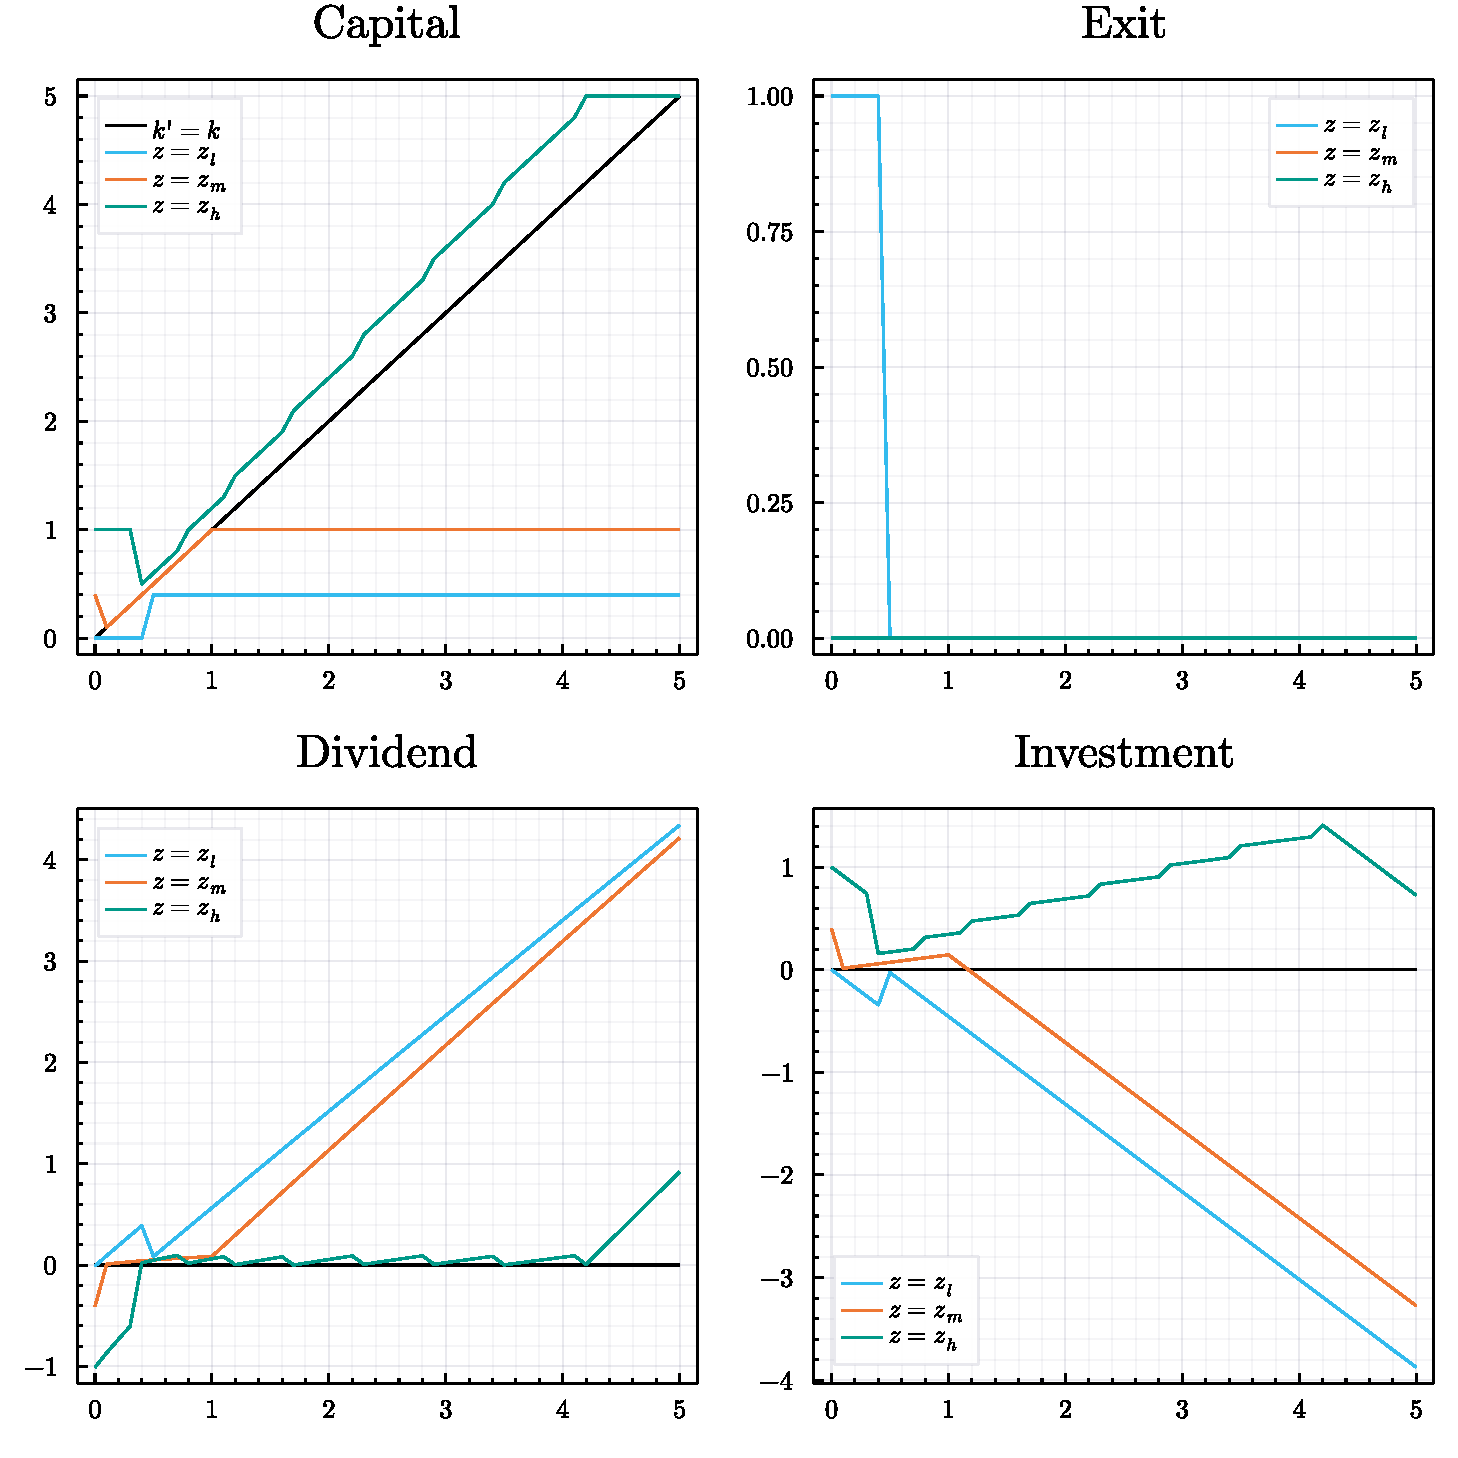
\includegraphics[scale=0.61]{pol_funcs.pdf}
    \end{figure}
    \begin{figure}\caption{Cumulative Distribution Functions}\label{fig:cdfs}
        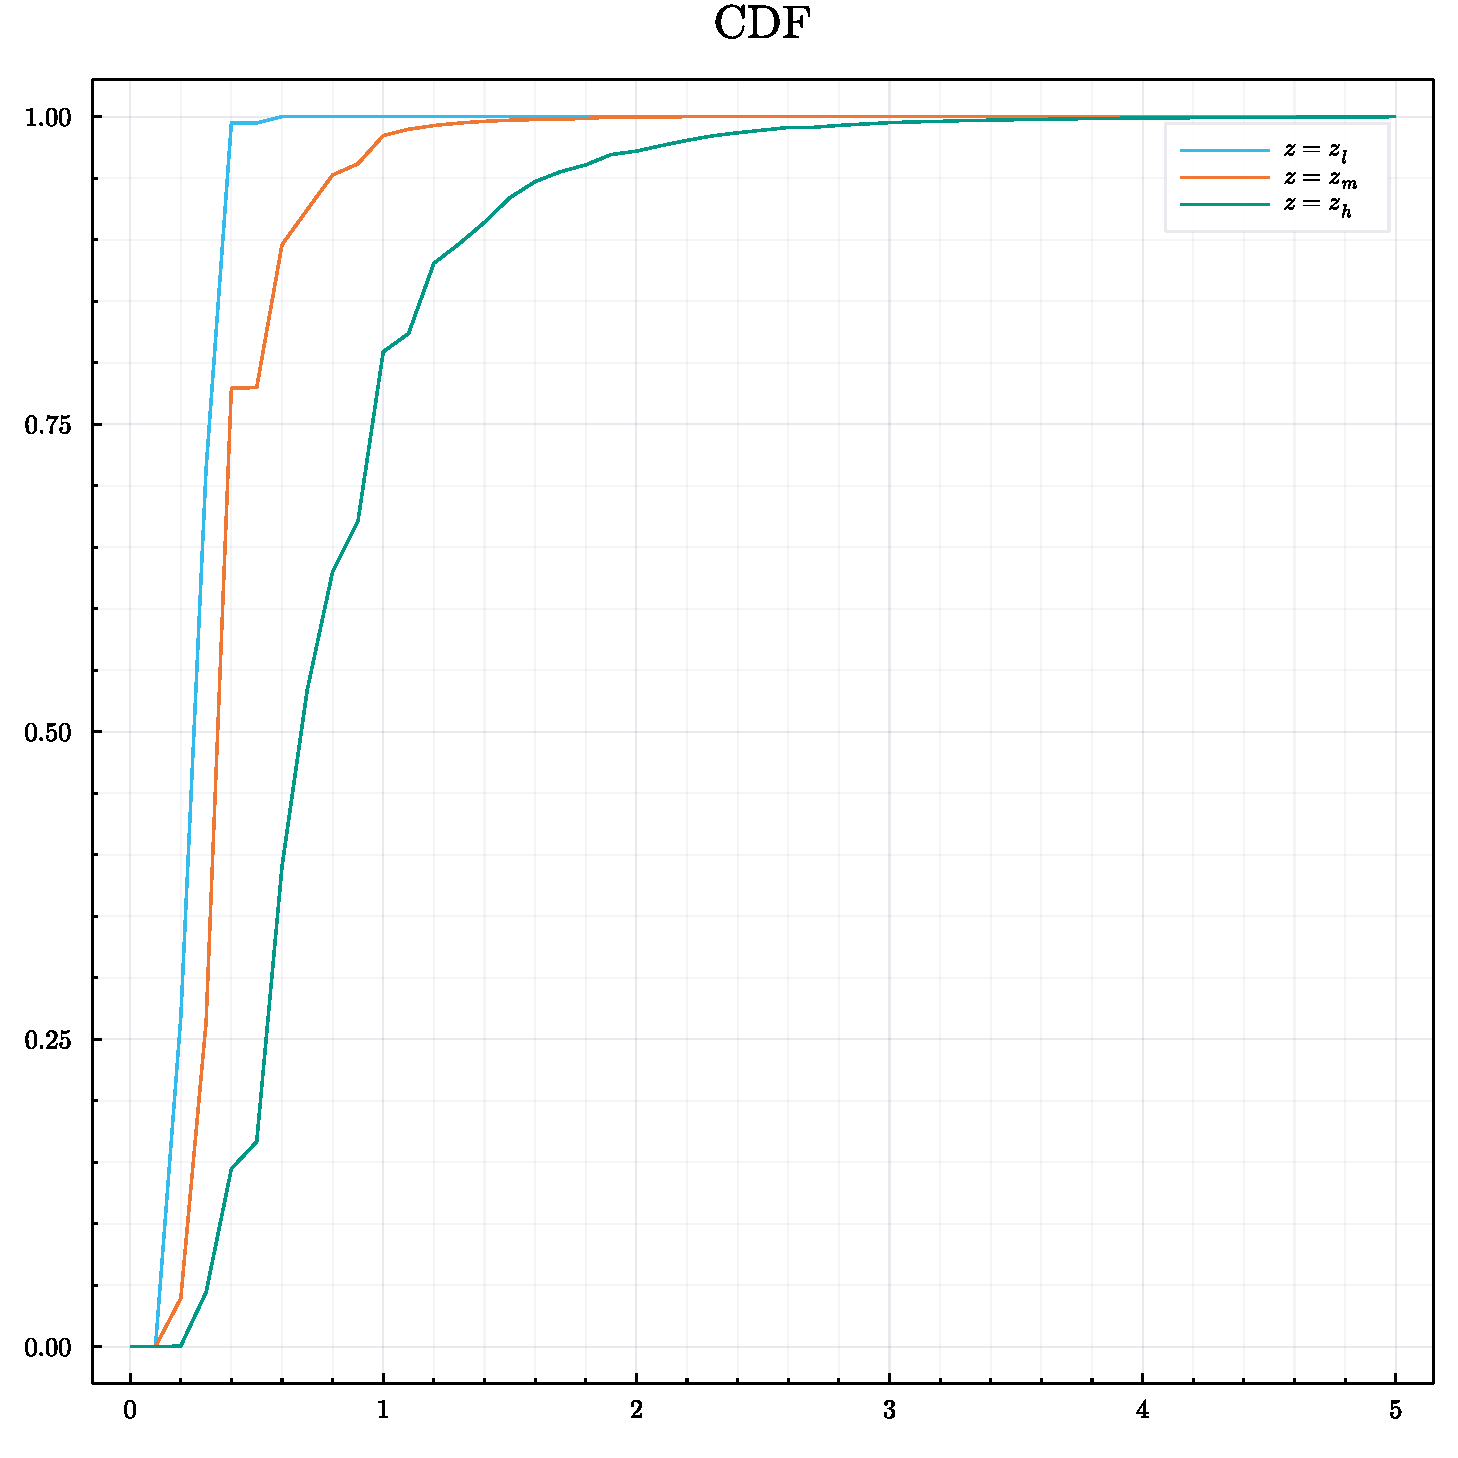
\includegraphics[scale=0.55]{cdf.pdf}
    \end{figure}
\end{answer}

\begin{exercise}
    Simulate the model creating a panel of 1200 firms for 10 years (save the shock processes). Then estimate the following equation
        $$
        \frac{i_{i, t}}{k_{i, t-1}}=b_{0}+b_{1} Q_{i, t-1}+b_{2} \frac{\pi_{i, t-1}}{k_{i, t-1}}+f_{t}+d_{i}+\epsilon_{i, t}
        $$
        where $Q_{i, t}$ is the Tobin's average $\mathrm{Q}$, defined as
        $$
        Q_{i, t}=\frac{p_{i, t}}{k_{i, t}}
        $$
    and report the results. Does the model make the same predictions as the regressions you ran on problem set 1 ?
\end{exercise}

\begin{answer}
    Regression results are bellow.
\end{answer}

\begin{exercise}
    Run a counterfactual where $\lambda_{0}=\lambda_{1}=0$ so that there are no financing frictions and create the same panel as above (using the same shock process). Is there cash-flow sensitivity?
\end{exercise}

\begin{answer}
    Regression results are bellow.
    \begin{table}\caption{Counterfactual Results}
        \begin{tabular}{lrr}
\toprule
                      &               \multicolumn{2}{c}{$i_{t}$}               \\ 
\cmidrule(lr){2-3} 
                      & Finantial Frictions (1) & No Finantial Frictions (2) \\ 
\midrule
$Q_{t-1}$             &                2.933*** &                    16.957*** \\ 
                      &                 (0.470) &                      (0.777) \\ 
$\pi_{t-1} / k_{t-1}$ &               -9.127*** &                    -8.632*** \\ 
                      &                 (1.709) &                      (1.445) \\ 
\midrule
FE Year               &                     Yes &                          Yes \\ 
FE Firm               &                     Yes &                          Yes \\ 
\midrule
Estimator             &                     OLS &                          OLS \\ 
\midrule
$N$                   &                   9,270 &                          519 \\ 
$R^2$                 &                   0.426 &                        0.937 \\ 
\bottomrule
\end{tabular}

    \end{table}

\end{answer}

\end{document}